

\documentclass[11pt]{article}
\usepackage[a4paper, total={6.5in,9in}]{geometry}

\usepackage[parfill]{parskip}    	
\usepackage{graphicx,caption,fancyhdr,xcolor,pdfpages,setspace}
\usepackage[hypertexnames=false]{hyperref}
\usepackage{minted}

\usepackage[english]{babel}
\usepackage[square,numbers]{natbib}
\bibliographystyle{abbrvnat}

\newcommand{\wrt}[1]{\mathrm{d}#1}
\newcommand{\bellforce}{Bell\hspace*{1.61803398875pt}\textbf{::}\hspace*{1.61803398875pt}Force}


\setlength{\fboxsep}{1em}

\hypersetup{
	colorlinks=true,
	linkcolor=darkgray,
	citecolor=red,
	urlcolor=red
}

\urlstyle{same}
\renewcommand{\footnoterule} % Push footnotes to the bottom of the page
	{\vfill\kern -3pt \hrule width 0.4\columnwidth \kern 2.6pt}

\makeatletter
\title{The \bellforce{}: An Innovative Dual-Engine Automotive Navigation System }
\let\Title\@title
\author{Y3862181}
\let\Author\@author
\date{Summer Term, 2023}
\let\Date\@date
\makeatother

\fancypagestyle{content}{
    \renewcommand{\headrulewidth}{0.4pt}
    \renewcommand{\footrulewidth}{0.4pt}
    \setlength{\headheight}{15pt}
    
	\fancyhf{}
	\fancyhead[L]{\Author}
	\fancyhead[R]{\bellforce{}}
	\fancyfoot[L]{\Date}
	\fancyfoot[R]{\thepage}
}
\onehalfspacing

\begin{document}
\begin{titlepage}
\centering
{\Huge Graph Theory Report}

\vspace{3cm}

\LARGE {The \bellforce{}: An Innovative Dual-Engine Automotive Navigation System}

\vspace{3cm}

{\LARGE Y3862181}

\vspace{2cm}



\vfill

{\itshape University of York}
\end{titlepage}

\titlepage
\tableofcontents

\pagestyle{content}
\maketitle

\section{Introduction}
\noindent
The \bellforce{} is a program in \texttt{C} that helps a driver find the most energy-efficient simple path given an origin and destination in a futuristic traffic system, whereby one can gain energy on certain routes. It comprises of a dual-engine, each used for a specific purpose. One engine is based on an exhaustive yet optimised brute-force algorithm, which always provides the most energy-efficient path, and the other is based on the much less resource-intensive modified Bellman-Ford algorithm, which provides a reasonable shortest path approximation.

This report will cover the justification behind the design of the program, crucial details regarding its implementation as well as an overview of the testing strategy adopted throughout its design.


\section{Design Rationale}
\subsection{The Graph}

According to the specification, the programmer is given data comprising of a list of routes, where each route specifies the origin, destination and energy expenditure between them. These routes must be bidirectional and some routes expend negative energy, meaning that there is an energy gain when driving through them. The network of routes can be modeled as a graph abstract data type (\texttt{ADT}), whereby the origin and destination values represent the vertices of the graph (V), the routes themselves represent the edges between these vertices (E), and the energy expenditure associated with each route represents the weight of its corresponding edge. A graph \texttt{ADT} is usually represented with either an adjacency list or an adjacency matrix abstract data structure (\texttt{ADS}). Both types of lists have their own pros and cons. The time complexity for building an adjacency matrix is $\mathcal{O}(V^2)$, whereas the time complexity for building an adjacency list is only $\mathcal{O}(E)$\cite{Sedgewick}. On the flip side, the time complexity for accessing an edge in an adjacency matrix is $\mathcal{O}(1)$, which is superior to the time complexity of accessing an edge in an adjacency list ($\mathcal{O}(E)$)\cite{Sedgewick}. It may therefore seem difficult to decide based on time complexity alone which list is worth implementing but when it comes to memory complexity, the nature of the graph will quickly determine which list is appropriate for a given design.

Due to memory considerations, an adjacency list is usually implemented in sparse graphs while an adjacency matrix is usually implemented in dense graphs. This is simply because the space complexity of an adjacency matrix is $\mathcal{O}(V^2)$, while an adjacency list has a better memory complexity of $\mathcal{O}(V + E)$\cite{Sedgewick}. The graph model for the current specification is fairly sparse, since it contains only 100 edges given 24 vertices, so an adjacency list was confidently selected over an adjacency matrix to improve the overall memory footprint of the program.

\subsection{The Algorithms}
In graph theory, whenever a route is bidirectional and the weight associated with it is of a negative value, a negative cycle is created by default. This means that the programmer is implicitly told from the specification alone that the graph is replete with negative cycles. The challenge with the specification is that it is theoretically intractable to compute an accurate single source shortest path (\texttt{SSSP}) for an arbitrary graph containing negative cycles\cite{Sedgewick}. This means that in order to have full confidence that the \texttt{SSSP} for any given graph is accurate, an inefficient algorithm with respect to both time and memory complexity must be implemented. Since in a fully connected graph, there are V amount of vertices, and since it is possible that the path could be as long as V number of edges without having revisited a vertex, the time complexity in the worst case scenario is $\mathcal{O}(V^V)$. This entails that the space complexity must also be $\mathcal{O}(V^V)$ since this would represent the amount of possible shortest paths required to be evaluated at run-time. In practice, since the brute-force algorithm implemented in the \bellforce{} is based on a Depth-first search algorithm with backtracking, it is possible to optimise the computation by getting rid of invalid paths during the exhaustive search of all possible paths and by limiting the list of valid simple paths to the number of record low energy expenditure paths (see \texttt{dfs\_rec} function in \texttt{brute\_force.c}). This, however, does not change the fact that the algorithm is still highly inefficient compared to a polynomial time shortest path algorithm, which is evidently a problem, since not all computing systems (especially embedded systems installed in automobiles) would be able to handle such an expensive time and memory complexity. Furthermore, from a scalability perspective, $\mathcal{O}(V^V)$ time and space complexity is an impractical choice so an alternative to such a predicament is necessary to avoid a potential computational impasse. 

This is precisely why the \bellforce{} features a second engine, which attempts to resolve the issue to some extent. Instead of using the stock Bellman-Ford directly on the original graph, the same graph albeit limited to directional negative edges is evaluated. In fact, a specific modulo pattern for evaluating directional negative edges was discovered while analysing the graph using \texttt{Mathematica}, which resulted in the exact same answers provided by the accurate yet inefficient brute-force algorithm for the routes provided by the specification (see \texttt{adjacency\_list\_constructor} function in \texttt{bellman\_ford.c}). Using this discovered modulo pattern on every possible unseen city-pair for the graph, however, does not guarantee accurate results, and will definitely not get rid of negative cycles on any given graph. The benefits of such implementation, however, are non-trivial. The Bellman-Ford algorithm has a worst-case time complexity of $\mathcal{O}(V * E)$  and a worst-case memory complexity of $\mathcal{O}(V)$\cite{Sedgewick}. This is due to its relaxation techniques, which efficiently evaluate the shortest path by iterating through the edges V - 1 times (at most) rather than relying on backtracking techniques (see \texttt{sp\_algorithm} function in \texttt{bellman\_ford.c}). Thus for less accurate results, it is possible to compute a reasonable \texttt{SSSP} in polynomial time without sacrificing a significant memory footprint. Both engines now have a purpose, and the user is able to choose efficiency over accuracy depending on the situation at hand. 
\subsection{Additional Data Structures}
Since the \bellforce{} incorporates both an exponential and a polynomial time \texttt{SSSP} algorithm, a versatile doubly linked list \texttt{ADS} was chosen in order to accommodate for a wide range of operations that will encompass the requirements for both implementations. For instance, in both the optimised brute-force and modified Bellman-Ford algorithms employed in the \bellforce{}, access to both the previous and next node of a linked list as well as the head and the tail of that list improves the overall time complexity of the program. Or in technical jargon, for a relatively trivial increase in memory footprint, the time complexity for adding and removing a node from a doubly linked list is $\mathcal{O}(1)$ whereas it would be $\mathcal{O}(n)$ in a singly linked list, where n represents the number of nodes in a given list.

In addition to a doubly linked list, a simple Dictionary \texttt{ADT} that assigns a key integer for every unique city that is read from the text file in the provided specification has been represented and implemented as an associative array ADS (see \texttt{strings\_table.c}). The increase in memory footprint of $\mathcal{O}(V)$ for constructing the associative array is negligible compared to the amount of memory allocation that the \texttt{SSSP} algorithms would require if strings were the default data type (particularly for the brute-force algorithm), with the added benefit that the access time for retrieving the string is only $\mathcal{O}(1)$. It is also non-trivial that a string in \texttt{C} is represented as an array of characters, thus using pointers for something that can be represented with a single integer might unnecessarily over-complicate the design of the \bellforce{}. 



\section{Program Architecture}

Since the \bellforce{} can operate with both an optimised brute-force and a modified Bellman-Ford algorithm, careful consideration regarding its program architecture is required in order to maintain an acceptable level of abstraction throughout its design. \autoref{fig:flowchart1} illustrates a high-level overview of the program architecture. It can be observed in \autoref{fig:flowchart1} that only common functions necessary for the implementation of both algorithms are exposed to the client while the functions associated with each algorithm are kept encapsulated. The way this was achieved was by giving \texttt{main.c} access to header files such as \texttt{algorithm.h} and \texttt{graph.h}, instead of direct access to the \texttt{brute\_force.c} and \texttt{bellman\_ford.c} implementation files. This fairly abstract interface enables the client to pick and choose whichever algorithm they desire to employ, without having to worry about the way they are implemented. The main drawback of this design, however, is that in order to keep those two algorithms encapsulated, quite a lot of non-abstract Getter and Setter functions in both \texttt{graph.h} and \texttt{list.h} had to be implemented, thereby sacrificing encapsulation with respect to the \texttt{ADS}s themselves. The reason this occurred is mainly because the optimised brute-force and the modified Bellman-Ford algorithms were individually designed prior to attempting to bridge them together. As a result, the amount of \texttt{ADS}-specific Getter and Setter functions required to keep both of these algorithms decluttered was higher than expected and thus sacrificed some abstraction. 
 

\begin{figure}[ht]
    \centering
    \fbox{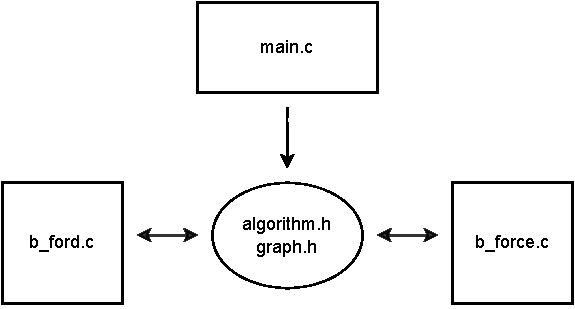
\includegraphics[width=0.8 \textwidth]{flowchart1.pdf}}
    \caption{The \bellforce{} Program Architecture.}
    \label{fig:flowchart1}
\end{figure}
\section{C-Centric Considerations}
\subsection{Memory Leaks}
Since \texttt{C} is not equipped with a garbage collector, hazardous memory leaks are bound to occur without thorough memory debugging. With the use of \texttt{valgrind} (an excellent memory leak debugger), it is possible to confirm that every single memory allocated during the program execution has been freed before returning from \texttt{main}. For completeness, proof that all memory allocated for both the optimised brute-force and the modified Bellman-Ford algorithms has been successfully deallocated can be viewed in both \texttt{Brute-Force Valgrind Report} and \texttt{Bellman-Ford Valgrind Report} presented below in consecutive order: 
\begin{minted}{text}
--------------------------------------------------------------------------
==2418== Command: bin/brute_force data/energy-v23-1.txt data/citypairs.txt
==2418== HEAP SUMMARY:
==2418==     in use at exit: 0 bytes in 0 blocks
==2418==   total heap usage: 1,889,043 allocs, 1,889,043 frees, 
            45,391,264 bytes allocated
==2418== 
==2418== All heap blocks were freed -- no leaks are possible
--------------------------------------------------------------------------
\end{minted}
\begin{minted}{text}
==2183== Command: bin/bellman_ford data/energy-v23-1.txt data/citypairs.txt
==2183== HEAP SUMMARY:
==2183==     in use at exit: 0 bytes in 0 blocks
==2183==   total heap usage: 1,150 allocs, 1,150 frees, 
            79,440 bytes allocated
==2183== 
==2183== All heap blocks were freed -- no leaks are possible
--------------------------------------------------------------------------
\end{minted}
It can also be observed in the report that the amount of memory allocated for the brute-force algorithm is a gargantuan amount of 45,391,264 bytes, which is three orders of magnitude bigger than the 79,440 bytes allocated for the modified Bellman-Ford algorithm. This highly correlates with our previous memory complexity analysis for both algorithms and justifies the necessity of having a dual-engine implementation in the \bellforce{}.

\subsection{Error and Exception Handling} 
Another testing feature \texttt{C} is sadly missing is an internal exception/error handler. Without an exception/error handler, the program, for instance, may abruptly crash due to a parsing error or a stack overflow without being able to detect where it occurred as well as exiting the program prior to freeing all the already allocated memory. To combat such hazardous behaviour, a custom error/exception handler can be accessed from \texttt{main.c} via \texttt{error.h} and implemented in \texttt{error.c} using an \texttt{enum} containing various error fields such as parsing errors (\texttt{STATUS\_PARSE}), system errors 
(\texttt{STATUS\_ERRNO}), and even a negative cycle detection error (\texttt{STATUS\_NEGCYCLE}), so that whenever a bug occurs in the program, the error will only be displayed after exiting from \texttt{main.c} and indicate the type of error that had occurred onto \texttt{stderr}. 

\section{Debug Mode}
Besides undergoing thorough memory leak debugging using \texttt{valgrind} and improving the robustness of the \bellforce{} via an implementation of a custom error/exception handler, an additional debugging mode feature can be accessed via \texttt{error.h} and implemented in \texttt{error.c} when choosing either \texttt{Brute-Force Debug} or \texttt{Bellman-Ford Debug} mode. If one of the debug modes is chosen, valuable additional data is displayed onto \texttt{stdout}. It can be observed that when either \texttt{Brute-Force Debug} or \texttt{Bellman-Ford Debug} modes is chosen, once the graph has been successfully constructed, the number of cities and routes represented in the graph is displayed onto \texttt{stdout}. In addition, it is possible to view the complete strings table as well as a carefully formatted adjacency list representing the graph network. All of these additional offerings are not merely eye-candy for the client. They were designed incrementally with agile development in mind, at every phase of the design. In other words, tests were conducted to ensure that the number of cities and routes matched the specification, that the strings table was built successfully and that the adjacency list correctly represented the network of the graph. What's more, making sure that most of the debugging features will be evaluated by the processor directives rather than the compiler further optimises the run-time performance of the \bellforce{} regardless of the chosen mode.   

\section{Results}

It can be seen in both \texttt{Brute-Force} and \texttt{Bellman-Ford} modes what the required \texttt{SSSP}s are including the total energy expenditure required for each path but it is also displayed below for ease of access: 

\begin{minted}{text}
Shortest Path Results
---------------------

Manchester -> Sheffield -> Nottingham -> Birmingham -> Liverpool -> Carlisle -> 
Moffat -> Glasgow -> Edinburgh -> Perth
Total expenditure: 65

Liverpool -> Carlisle -> Manchester -> Sheffield -> Leeds -> York -> Whitby
Total expenditure: -135

Lincoln -> Sheffield -> Nottingham -> Birmingham
Total expenditure: 58
\end{minted}
For each algorithm mode, the corresponding time it takes to compute the three \texttt{SSSP}s is also displayed onto \texttt{stdout}: 0.24 seconds for brute-force and 0.003 seconds for Bellman-Ford. This highly correlates with our previous time complexity analysis for both algorithms and justifies the necessity of having a dual-engine implementation in the \bellforce{}.

\bibliography{bib}

\section{Appendix}
\subsection{main.c}
\label{ssec: main.c}
\begin{minted}{c}
/* The Bell::Force, written by Y3862181 */

#include <stdio.h>
#include <stdlib.h>
#include <string.h>

#include "algorithm.h"
#include "graph.h"
#include "strings_table.h"
#include "error.h"
#include "time.h"

/* Prints a salutation that corresponds to the chosen algorithm
 * during link-time */
static void print_welcome ( void )
{
    puts ( "Welcome to the Bell-Force traffic manager..." );

#ifdef ALG_BELLMAN_FORD
    puts ( "... compiled with the Bellman-Ford algorithm!" );
#else
    puts ( "... compiled with the recursive depth-first search algorithm!" );
#endif

    print_debug ( "Debugging mode is enabled." );
    putchar ( '\n' );
}

/* Prints a generic farewell message */
static void print_goodbye ( void )
{
    puts ( "Thank you for using the Bell-Force traffic manager. " \
           "Enjoy your optimised journey!" );
}


/* opening all the required files for the program by assigning each
 * expected file name to its corresponding argument, simulating their
 * invocation by the command line. Error-handling is implemented in
 * case the wrong file name is invoked or if a file is missing */
static enum status open_files ( FILE * * fpdata, FILE * * fpsearch,
    FILE * * fpout, int argc, char * * argv )
{
    char * const ENERGY_DEFAULT = "energy-v23-1.txt";
    char * const PAIRS_DEFAULT  = "citypairs.txt";
    char * const OUTPUT_DEFAULT = "output.txt";

    char * energy_path = ENERGY_DEFAULT, * pairs_path = PAIRS_DEFAULT,
        * output_path = OUTPUT_DEFAULT;

    if ( argc >= 2 )
        energy_path = argv [ 1 ];
    if ( argc >= 3 )
        pairs_path  = argv [ 2 ];
    if ( argc >= 4 )
        output_path = argv [ 3 ];

    if ( ! ( * fpdata = fopen ( energy_path, "r" ) ) ) {
        report_error ( STATUS_ERRNO, energy_path );
        return STATUS_ERRNO;
    }
    if ( ! ( * fpsearch = fopen ( pairs_path, "r" ) ) ) {
        fclose ( * fpdata );
        report_error ( STATUS_ERRNO, pairs_path );
        return STATUS_ERRNO;
    }
    if ( ! ( * fpout = fopen ( output_path, "w" ) ) ) {
        fclose ( * fpdata   );
        fclose ( * fpsearch );
        report_error ( STATUS_ERRNO, output_path );
        return STATUS_ERRNO;
    }
    return STATUS_OK;
}

/* closing all the required files for the program */
static void close_files ( FILE * * fpdata, FILE * * fpsearch,
    FILE * * fpout )
{
    fclose ( * fpout    );
    fclose ( * fpsearch );
    fclose ( * fpdata   );
}

int main ( int argc, char * * argv )
{
    FILE * fpdata = NULL, * fpsearch = NULL, * fpout = NULL;
    struct Strings_table * table = NULL;
    struct Graph * graph = NULL;
    enum status status = STATUS_OK;

    /* Prints a salutation that corresponds to the chosen algorithm
     * during link-time */
    print_welcome ( );

    /* opening all the required files for the program */
    if ( open_files ( & fpdata, & fpsearch, & fpout, argc, argv )
            != STATUS_OK )
        return EXIT_FAILURE;

    /* Constructs a strings table that will be used in order to convert
     * the string values of the cities into numbers to optimise computation
     * and facilitate implementation of the program. Error-handling is
     * implemented in case memory for the table has not been allocated
     * successfully */
    if ( ( status = table_constructor ( & table ) ) != STATUS_OK ) {
        report_error ( STATUS_ERRNO, "Could not initialise " \
            "the strings table." );
        close_files ( & fpdata, & fpsearch, & fpout );
        return EXIT_FAILURE;
    }

    
    
    /* Constructs the graph as well as its adjacency list. Error-handling
     * is implemented so that if there has either been a parsing error
     * while building the graph or if memory for the graph has not been
     * allocated successfully, then the program will not quit abruptly
     * and the specific error type and cause of error will be reported */
    if ( ( status = graph_constructor ( & graph, fpdata, table ) )
            != STATUS_OK ) {
        report_error ( status, "Could not construct the graph." );
        close_files ( & fpdata, & fpsearch, & fpout );
        return EXIT_FAILURE;
    }

    /* In Debug mode, print confirmation that the graph was
     * constructed successfully and indicate the amount of cities
     * and routes contained in the graph */
    printf_debug ( "\nGraph was created successfully. It contains " \
        "%u cities and %u routes.\n\n", graph_get_num_cities ( graph ),
        graph_get_num_routes ( graph ) );

    /* In Debug mode, print the strings table */
    table_print ( table );

    /* In Debug mode, print the adjacency list information. */
    display_adjacency_list ( graph, table );

    /* Initialising variables for computing the time taken
     * to output the shortest path */
    double time_start, time_end, elapsed_time_seconds;
    time_start = ( double ) clock ( );










    /* Displays onto the terminal as well as outputs to a text
     * file the entire shortest path between given origin and
     * destination as well as its total energy expenditure. Error-handling
     * is implemented so that if memory has not been allocated
     * successfully during the computation or if a negative cycle is
     * detected, instead of quitting the program abruptly, the specific
     * error type and cause of error will be reported */
    puts ( "Shortest Path Results\n---------------------\n" );
    if ( ( status = shortest_path ( fpsearch, graph, table, fpout ) )
           != STATUS_OK ) {
        graph_destructor ( graph );
        table_destructor ( table );
        report_error ( status, "Could not compute the shortest path." );
        close_files ( & fpdata, & fpsearch, & fpout );
        return EXIT_FAILURE;
    }

    /* Displays the time it took to compute shortest-path */
    time_end = ( double ) clock ( );
    elapsed_time_seconds = ( double ) ( time_end - time_start )
        / CLOCKS_PER_SEC;
    printf ( "\nTotal computation time: %f seconds.\n", elapsed_time_seconds );

    /* Destroys the graph, strings table and closes the files after program
     * was executed successfully */
    graph_destructor ( graph );
    table_destructor ( table );
    close_files ( & fpdata, & fpsearch, & fpout );

    /* Prints a generic farewell message */
    print_goodbye ( );

    return EXIT_SUCCESS;
}
\end{minted}
\newpage
\subsection{error.h}
\begin{minted}{c}
#ifndef ERROR_H
#define ERROR_H

/* This file contains access to all of the debugging and error-handling
 * features of the program. By enabling BF_DEBUG during link-time, all the
 * debugging print statements will be evaluated during the compilation
 * phase rather than during the execution phase for optimal performance.
 * Error-handling is implemented via an enum called status, which
 * enumerates the types of errors that are expected to occur
 * during run-time. Stylistic ideas for the syntactic implementation of
 * the debugger came from https://stackoverflow.com/a/154138 */

#ifdef BF_DEBUG

#include <stdio.h>

#define print_debug(str) fputs ( str, stderr )

#define putchar_debug(chr) fputc ( chr, stderr )

#define printf_debug(fmt, ...) fprintf ( stderr, fmt, __VA_ARGS__ )

#define println_debug(str)          \
    do {                            \
            fputs ( str,  stderr ); \
            fputc ( '\n', stderr ); \
    } while ( 0 )

#else

#define print_debug(str)
#define putchar_debug(chr)
#define printf_debug(fmt, ...)
#define println_debug(str)

#endif /* BF_DEBUG */


/* enumerates the types of errors that could potentially occur
 * during run-time */
enum status {
        STATUS_OK,       /* Success        */
        STATUS_ERRNO,    /* System error   */
        STATUS_NEGCYCLE, /* Negative cycle */
        STATUS_PARSE,    /* Parse error    */
};

/* Reports a specific error within the error-handling
 * category */
void report_error ( enum status, const char * );

#endif /* ERROR_H */
\end{minted}
\newpage
\subsection{error.c}
\begin{minted}{c}
#include <stdio.h>
#include <string.h>
#include <errno.h>

#include "error.h"


/* Contains all the error-handling categories required for
 * the program */
static const char * bf_strerror ( enum status code )
{
    switch ( code ) {
        case STATUS_OK:       return "All OK";
        case STATUS_ERRNO:    return strerror ( errno );
        case STATUS_NEGCYCLE: return "Negative cycle detected";
        case STATUS_PARSE:    return "File parse error";

        default:              return "Unknown error code";
    }
}

/* Reports a specific error within the error-handling
 * category */
void report_error ( enum status code, const char * message )
{
    fputs ( "Error: ", stderr );
    fputs ( bf_strerror ( code ), stderr );

    if ( message ) {
        fputs ( ": ", stderr );
        fputs ( message, stderr );
    }

    fputc ( '\n', stderr );
}
\end{minted}
\newpage
\subsection{strings\_table.h}
\begin{minted}{c}
#ifndef STRINGS_TABLE_H
#define STRINGS_TABLE_H

#include <stddef.h>
#include <stdbool.h>
#include "error.h"


/* A basic Dictionary ADT implemented
 * as an associative array that stores a string
 * value and a key that is associated with it */
struct Strings_table;

/* Construct the strings table, ensuring sufficient memory to accommodate
 * default city names. Error-handling is implemented in case memory has not
 * been allocated successfully */
enum status table_constructor ( struct Strings_table * * );

/* Free all memory allocated in the given strings table. */
void table_destructor ( struct Strings_table * );

/* Adds a new city name to the strings table */
unsigned int table_add ( struct Strings_table *, char * );

/* Debug mode only: prints the entire strings table */
void table_print ( struct Strings_table * );

/* Returns an index value corresponding to a given string. If the
 * string value does not match any of the values contained in the table,
 * an error is reported */
unsigned int table_search ( struct Strings_table *, char * );

/* Returns a string value corresponding to a given index number */
char * table_get ( struct Strings_table *, unsigned int );

/* Enabling an error flag in the table */
bool table_get_error ( struct Strings_table * );

/* Clearing an error flag in the table */
void table_clear_error ( struct Strings_table * );

#endif /* STRINGS_TABLE_H */
\end{minted}
\newpage
\subsection{strings\_table.c}
\begin{minted}{c}
#include <stdlib.h>
#include <stdio.h>
#include <string.h>
#include <stdbool.h>
#include <errno.h>

#include "strings_table.h"
#include "error.h"

/* A basic Dictionary ADT implemented
 * as an associative array that stores a string
 * value and a key that is associated with it */
struct Strings_table {
    char * * data;
    unsigned int capacity;
    unsigned int size;
    bool error;
};

/* Free all memory allocated in the given strings table */
void table_destructor ( struct Strings_table * table )
{
    free ( table -> data );
    free ( table );
}


/* Enabling an error flag in the table */
bool table_get_error ( struct Strings_table * self )
{
    return self -> error;
}

/* Clearing an error flag in the table */
void table_clear_error ( struct Strings_table * self )
{
    self -> error = false;
}

/* Construct the strings table, ensuring sufficient memory to accommodate
 * default city names. Error-handling is implemented in case memory has not
 * been allocated successfully */
enum status table_constructor ( struct Strings_table * * in_table )
{
    const unsigned int DEFAULT_TABLE_CAPACITY = 32;
    struct Strings_table * table = NULL;

    /* Allocates memory for the table superstructure and string addresses */
    if ( ! ( table = malloc ( sizeof ( struct Strings_table ) ) ) ||
            ! ( table -> data = malloc ( sizeof ( char * ) *
            DEFAULT_TABLE_CAPACITY ) ) ) {
        free ( table );
        return STATUS_ERRNO;
    }

    table -> capacity = DEFAULT_TABLE_CAPACITY;
    table -> size = 0;

    * in_table = table;
    return STATUS_OK;
}

/* Adds a new city name to the strings table */
unsigned int table_add ( struct Strings_table * self, char * str )
{
    self -> data [ self -> size++ ] = str;
    return self -> size - 1;
}

/* Debug mode only: prints the entire strings table */
void table_print ( struct Strings_table * self )
{
    print_debug ( "\nStrings Table\n---------------\n");
    for ( unsigned int i = 0; i < self -> size; i++ )
        printf_debug ( "#%02u\t\"%s\"\n", i, self -> data [ i ] );
    putchar_debug ( '\n' );
}

/* Returns an index value corresponding to a given string. If the
 * string value does not match any of the values contained in the table,
 * it returns an error */
unsigned int table_search ( struct Strings_table * self, char * element )
{
    unsigned int i;

    for ( i = 0; i < self -> size; i++ )
        if ( strcmp ( self -> data [ i ], element ) == 0 )
            return i;

    self -> error = true;
    return 0;
}

/* Returns a string value corresponding to a given index number */
char * table_get ( struct Strings_table * self, unsigned int idx )
{
    return self -> data [ idx ];

}
\end{minted}
\newpage
\subsection{algorithm.h}
\begin{minted}{c}
#ifndef ALGORITHM_H
#define ALGORITHM_H

/* This file abstracts away the details of the each algorithm's
 * implementation by having two generic functions: "graph_constructor",
 * which constructs a graph that loads data from a given energy
 * text file and "sp_algorithm", which searches for a shortest path
 * between a given origin and destination read from a given city-pair
 * text file */

#include <stdio.h>

#include "error.h"
#include "graph.h"
#include "strings_table.h"

/* Algorithm-dependent implementations, determined at link-time */


/* Implementation-agnostic graph constructor */
enum status graph_constructor ( struct Graph * *, FILE *,
    struct Strings_table * );

/* Implementation-agnostic single source shortest path algorithm */
enum status sp_algorithm ( struct Graph *, unsigned int, unsigned int,
    struct Strings_table *, FILE * fpout );

#endif /* ALGORITHM_H */
\end{minted}
\newpage
\subsection{brute\_force.c}
\begin{minted}{c}
#ifdef ALG_BRUTE_FORCE
#undef ALG_BELLMAN_FORD
#endif

#ifdef ALG_BELLMAN_FORD
#error "To use brute-force, undefine ALG_BELLMAN_FORD."
#endif

#include <limits.h>
#include <stdlib.h>

#include "list.h"
#include "graph.h"

#include "algorithm.h"

/* Gets an energy value by providing the origin and destination of a current
 * edge. This function returns 0 if the partial solution is empty */
static int get_energy ( struct List * p_sol, struct Graph * self,
    unsigned int dest )
{
    struct Node * head_next;
    unsigned int origin;

    if ( !list_is_empty ( p_sol ) ) {

        origin = get_tail_city ( p_sol );

        head_next = graph_get_adj_head ( self, origin );

        while ( node_get_city ( node_get_next ( head_next ) ) != dest &&
                node_get_next ( head_next ) )
            head_next = node_get_next ( head_next );

        return node_get_energy ( node_get_next ( head_next ) );
    }
    return 0;
}

/* Exhaustive depth-first search algorithm, which keeps track
 * of the routes which had already been visited. Error-handling is
 * implemented in case memory has not been allocated successfully
 * during the computation */
static enum status dfs_rec ( struct Graph * self, unsigned int origin,
    unsigned int dest, struct List * p_sol, struct Simple_paths * sp,
    int * min_sum )
{
    int sum;
    struct Node * head = graph_get_adj_head ( self, origin );
    enum status status = STATUS_OK;

    /* The city has already been visited; nothing to do */
    if ( node_is_visited ( head ) )
        return status;

    /* If we have reached the destination, commit the complete path
     * (represented by the partial solution) to the list of simple paths */
    if ( node_get_city ( head ) == dest ) {

        if ( ( status = list_append ( p_sol, node_get_city ( head ),
            get_energy ( p_sol, self, node_get_city ( head ) ) ) ) != STATUS_OK )
            return status;

        /* Evaluates whether the new valid path is more efficient than the
         * previous ones and if so it is added to the list of simple paths */
        sum = list_get_energy_sum ( p_sol );
        if ( sum < ( * min_sum ) ) {
            * min_sum = sum;
            if ( ( status = add_simple_path ( sp, p_sol ) ) != STATUS_OK )
                return status;
        }

        /* Removes the last element from the partial solution list to ensure that
         * the current path is updated correctly */
        remove_last_element ( p_sol );
        return status;
    }

    /* Otherwise, mark the city as visited and append its path to the
     * partial solution list */
    node_set_visited ( head, true );

    if ( ( status = list_append ( p_sol, node_get_city ( head ),
        get_energy ( p_sol, self, node_get_city ( head ) ) ) ) != STATUS_OK )
        return status;

    /* We recurse over all cities reachable from the current node */
    while ( node_get_next ( head ) ) {

        if ( ( status = dfs_rec ( self,
            node_get_city ( node_get_next ( head ) ), dest, p_sol, sp,
            min_sum ) ) != STATUS_OK )
            return status;

        head = node_get_next ( head );

        if ( ! node_get_next ( head ) )
            node_set_visited ( graph_get_adj_head ( self,
                node_get_adj_idx ( head ) ), false );
    }

    /* Removes the last element from the partial solution list so that the
       current path will be updated correctly and in order to free unused data */
    if ( get_list_length ( p_sol ) > 1 )
        remove_last_element ( p_sol );

    return status;
}








/* constructs the adjacency lists for the graph. Error-handling is implemented
 * in case memory has not been allocated successfully while building the
 * adjacency lists */
static enum status adjacency_list_constructor ( struct Graph * graph )
{
    enum status status = STATUS_OK;

    unsigned int num_routes = graph_get_num_routes ( graph );
    if ( ( status = adjacency_list_internal_constructor ( graph ) )
            != STATUS_OK )
        return status;

    for ( unsigned int i = 0; i < num_routes; i += 2 )
        if ( ( status = make_directed_node ( graph, i, i + 1 ) ) != STATUS_OK
                || ( status = make_directed_node ( graph, i + 1, i ) )
                != STATUS_OK )
            return status;

    return status;
}

/* Displays the shortest path as well as its total energy expenditure.
 * In addition, it outputs the specified shortest path to a text file
 * including the required total energy expenditure */
void display_shortest_path ( struct Simple_paths * sp,
    struct Strings_table * table, FILE * fpout )
{
    display_path ( sp_get_tail ( sp ), table, true );
    output_path ( sp_get_tail ( sp ), table, true, fpout );
    printf ( "Total expenditure: %d\n\n",
        list_get_energy_sum ( sp_get_tail ( sp ) ) );
    fprintf ( fpout, "Total expenditure: %d\n\n",
        list_get_energy_sum ( sp_get_tail ( sp ) ) );
}





/* Constructs the graph with its corresponding adjacency list. Error-handling
 * is implemented in case a parsing error has occurred during the loading of
 * the graph or memory has not been allocated successfully for
 * the graph as well as for its embedded adjacency list */
enum status graph_constructor ( struct Graph ** in_graph, FILE * fp,
    struct Strings_table * table )
{
    enum status status = STATUS_OK;
    struct Graph * graph = NULL;

    if ( ( status = graph_internal_constructor ( &graph, fp, table ) )
            != STATUS_OK || ( status = adjacency_list_constructor ( graph ) )
            != STATUS_OK )
        return status;

    * in_graph = graph;
    return status;
}

/* Computes and outputs the shortest path between a given origin and
 * destination. Error-handling is implemented in case memory has not been
 * allocated successfully during the computation */
enum status sp_algorithm ( struct Graph * self, unsigned int origin,
    unsigned int destination, struct Strings_table * table, FILE * fpout ) {

    enum status status = STATUS_OK;
    struct List * p_sol = NULL;
    struct Simple_paths * sp = NULL;

    if ( ( status = list_constructor ( & p_sol ) ) != STATUS_OK )
        return status;

    if ( ( status = simple_paths_constructor ( & sp ) ) != STATUS_OK ) {
        list_destructor ( p_sol );
        return status;
    }



    /* Used to record the shortest path so that it would not be necessary
     * to add unnecessary valid simple paths to the simple paths list */
    int min_sum = INT_MAX;

    /* Inefficient yet accurate depth first search with backtracking algorithm
     * capable of getting an exact shortest path for a graph containing negative
     * cycles */
    if ( ( status = dfs_rec ( self, origin, destination, p_sol, sp, & min_sum ) )
            != STATUS_OK )
        return status;

    /* Displays the shortest path as well as its total energy expenditure.
     * In addition, it outputs the specified shortest path to a text file
     * including the required total energy expenditure */
    display_shortest_path ( sp, table, fpout );

    list_destructor ( p_sol );

    simple_paths_destructor ( sp );

    return status;
}
\end{minted}
\newpage
\subsection{bellman\_ford.c}
\begin{minted}{c}
#ifndef ALG_BELLMAN_FORD
#error "To use Bellman-Ford, define ALG_BELLMAN_FORD."
#endif

#include <stdio.h>
#include <stdlib.h>
#include <string.h>
#include <stdbool.h>
#include <ctype.h>

#include "graph.h"
#include "list.h"
#include "strings_table.h"

#include "algorithm.h"

#define BF_INFINITY ( 1000 )

/* Construct a modified adjacency list according to the requirements of the
 * Bellman-Ford algorithm. A modulo pattern is created such that only the
 * directed negative edges are evaluated. Error-handling is implemented
 * in case memory has not been allocated successfully */
static enum status adjacency_list_constructor ( struct Graph * graph )
{
    enum status status = STATUS_OK;

    const size_t num_routes = graph_get_num_routes ( graph );

    unsigned int neg_edges = 0, modulo = 5;
    bool forward_dir = true;
    int energy;

    if ( ( status = adjacency_list_internal_constructor ( graph ) )
            != STATUS_OK )
        return status;

    
    
    for ( unsigned int i = 0; i < num_routes; i += 2 ) {

        energy = route_get_energy ( graph, i );

        if ( energy > 0 ) {

            /* Case #1: The energy is positive. We add the route in the forward
             * direction and ignore the modulo pattern */

            if ( ( status = make_directed_node ( graph, i, i + 1 ) ) != STATUS_OK
                || ( status = make_directed_node ( graph, i + 1, i ) )
                != STATUS_OK )
            return status;

        } else if ( energy < 0 && forward_dir ) {

            /* Case #2: The energy is negative, and route is forward-going. We
             * add the route in the forward direction, and apply the modulo
             * pattern */

            if ( ( status = make_directed_node ( graph, i, i + 1 ) ) != STATUS_OK )
                return status;
            neg_edges++;

            if ( neg_edges == modulo ) {
                modulo--;
                neg_edges = 0;
                forward_dir = false;
            }
        } else {

            /* Case #3: The energy is negative, and the route is backward-going.
             * We add the route in the reverse direction, and apply the modulo
             * pattern */

            if ( ( status = make_directed_node ( graph, i + 1, i ) ) != STATUS_OK )
                return status;
            neg_edges ++;

            if ( neg_edges == modulo ) {
                modulo--;
                neg_edges = 0;
                forward_dir = true;
            }
        }
    }
    return status;
}

/* Initialises the origin city ID to 0 and the rest of the city IDs to
 * infinity. A value of 1000 has been defined to represent infinity to
 * prevent an overflow error during computation */
static void initialise_edges ( struct Graph * self, unsigned int origin )
{
    const unsigned int num_cities = graph_get_num_cities ( self );

    /* Initialise all the energies of the cities to infinity except for the
     * origin city */
    node_set_energy ( graph_get_adj_head ( self, origin ), 0 );

    for ( unsigned int i = 0; i < num_cities; i++ )
        if ( ! graph_nodes_equal ( self, i, origin ) )
            node_set_energy ( graph_get_adj_head ( self, i ), BF_INFINITY );
}

/* Continually relaxes each city ID value until the values associated with
 * each city ID reach a steady state. If during an iteration no updates to
 * any city ID value occur, the relaxation process will terminate to avoid
 * unnecessary iterations. */
static bool relax_edges ( struct Graph * self )
{
    const unsigned int num_cities = graph_get_num_cities ( self );
    bool update_detect = true;
    int energy_sum;

    
    
    
    /* The outer loop of the Bellman-Ford algorithm (iterates over all
     * of the vertices of the graph - 1 times) */
    for ( unsigned int i = 0; i < num_cities - 1 && update_detect; i++ ) {

        update_detect = false;
        /* The inner-loop of the Bellman-Ford algorithm (iterates over all
         * of the edges of the graph) */
        for ( unsigned int j = 0; j < num_cities; j++ )

            for ( struct Node * head = node_get_next ( graph_get_adj_head
                        ( self, j ) ); head;
                    head = node_get_next ( head ) ) {

                energy_sum = node_get_energy ( graph_get_adj_head ( self, j ) )
                    + node_get_energy ( head );

                /* If the value associated with the origin city ID +
                 * the energy required to get to the destination city ID is
                 * less than the current value associated with the destination
                 * city ID, update the value associated with the destination
                 * city ID with the value associated with the origin city ID +
                 * the energy required to get to the destination city ID */
                if ( energy_sum < node_get_energy ( graph_get_adj_head ( self,
                            node_get_city ( head ) ) ) ) {

                    node_set_energy ( graph_get_adj_head ( self, node_get_city
                        ( head ) ), energy_sum );
                    node_set_prev_city ( graph_get_adj_head ( self,
                        node_get_city ( head ) ), node_get_adj_idx ( head ) );

                    update_detect = true;
                }
            }
    }

    return ! update_detect;
}


/* Displays the shortest path taken from the origin to the destination
 * by first creating a list that represents the shortest path from the
 * destination to the origin. This step is required because of the way
 * the Bellman-Ford algorithm is implemented. It is only possible to
 * first retrieve the destination city ID and work backwards to find out
 * which previous city ID is part of the shortest path. While working
 * out all previous city IDs of the shortest path, when the prev city ID
 * matches the origin city ID, the list is completed. Once the list is
 * is complete, the shortest path will be displayed in reverse order
 * (to make the path appear non-reversed) in addition to the total energy
 * expenditure required for that path. Error-handling is implemented in case
 * memory could not be allocated for the list or if there is a negative cycle
 * contained in the graph */
static enum status display_bellman_ford_path ( struct Graph * self,
    unsigned int origin, unsigned int destination, struct List * p_sol,
    bool display_flag, struct Strings_table * table, FILE * fpout )
{
    enum status status = STATUS_OK;

    struct Node * head = graph_get_adj_head ( self, destination );

    if ( display_flag ) {

        /* Creating the reversed shortest path list */
        while ( node_get_city ( head ) != origin ) {

            if ( ( status = list_append ( p_sol, node_get_city ( head ), 0 ) )
                    != STATUS_OK )
                return status;

            head = graph_get_adj_head ( self, node_get_prev_city ( head ) );
        }

        if ( ( status = list_append ( p_sol, node_get_city ( head ), 0 ) )
                != STATUS_OK )
            return status;

        
        
        /* Displays the path onto stdout */
        display_path ( p_sol, table, false );

        /* Writes the path to output.txt */
        output_path ( p_sol, table, false, fpout );

        printf ( "Total expenditure: %d\n\n", node_get_energy (
            graph_get_adj_head ( self, destination ) ) );

        fprintf ( fpout, "Total expenditure: %d\n\n", node_get_energy (
                  graph_get_adj_head ( self, destination ) ) );
    }
    else
        return STATUS_NEGCYCLE;

    return status;
}

/* If ALG_BELLMAN_FORD is selected, we overload the algorithm functions with
 * Bellman-Ford implementations. Error-handling is implemented in case
 * the graph or its embedded adjacency list did not build successfully */
enum status graph_constructor ( struct Graph * * in_graph, FILE * fp,
                                struct Strings_table * table )
{
    enum status status = STATUS_OK;
    struct Graph * graph = NULL;

    if ( ( status = graph_internal_constructor ( &graph, fp, table ) )
           != STATUS_OK || ( status = adjacency_list_constructor ( graph ) )
           != STATUS_OK )
        return status;

    *in_graph = graph;
    return status;
}




/* If ALG_BELLMAN_FORD is selected, we overload the algorithm functions with
 * Bellman-Ford implementations. Error-handling is implemented in case
 * the shortest path list could not build successfully or if a negative
 * cycle is contained in the graph */
enum status sp_algorithm ( struct Graph * self, unsigned int origin,
    unsigned int destination, struct Strings_table * table, FILE *fpout )
{
    enum status status = STATUS_OK;

    int display_flag;

    struct List * p_sol = NULL;

    if ( ( status = list_constructor ( &p_sol ) ) != STATUS_OK )
        return status;

    /* initialise edges prior to relaxation */
    initialise_edges ( self, origin );

    /* Continually relaxing each city until no more
     * changes occur. Exit the loop when no relaxations are required after a full
     * linear search of all the routes. */
    display_flag = relax_edges ( self );

    /* Displays the shortest path as well as its total energy expenditure.
     * In case a negative cycle is detected, the program will terminate.
     * In addition, it outputs the specified shortest path to a text file
     * including the required total energy expenditure */
    if ( ( status = display_bellman_ford_path ( self, origin, destination, p_sol,
        display_flag, table, fpout ) ) != STATUS_OK ) {
        list_destructor ( p_sol );
        return status;
    }

    list_destructor ( p_sol );
    return status;
}
\end{minted}
\newpage
\subsection{graph.h}
\begin{minted}{c}
#ifndef GRAPH_H
#define GRAPH_H

#include <stdio.h>
#include <stdbool.h>

#include "strings_table.h"
#include "error.h"

#define MAX_CITY_LENGTH ( 32 )

/* Represents a graph ADT, which contains an array of adjacency
 * lists structs implemented with a doubly linked list ADS, and an array of
 * Route structs for storing the data loaded from the given text file implemented
 * with an array ADS */
struct Graph;

/* Represents a single node in the adjacency list of the graph */
struct Node;

/* Represents all of the data collected from the given text file */
struct Route;

/* Allocates memory for the internal graph. Error-handling is implemented
 * in case memory cannot be allocated for the superstructure of the internal
 * graph */
enum status graph_internal_constructor ( struct Graph * *, FILE *,
    struct Strings_table * );

/* Frees the remaining memory associated with the graph */
void graph_destructor ( struct Graph * );

/* Allocates memory for an array of adjacency lists */
enum status adjacency_list_internal_constructor ( struct Graph * );

/* Adds a directional route to the adjacency list. */
enum status make_directed_node ( struct Graph *, unsigned int,
    unsigned int );

/* Checks if the nodes are equal */
bool graph_nodes_equal ( struct Graph * self, unsigned int, unsigned int );

/* Gets the number of cities in the graph */
unsigned int graph_get_num_cities ( struct Graph * );

/* Gets the number of routes in the graph */
unsigned int graph_get_num_routes ( struct Graph * );

/* Gets the next value of the current node */
struct Node * node_get_next ( struct Node * );

/* Gets the head of a city ID index in the adjacency list */
struct Node * graph_get_adj_head ( struct Graph *, unsigned int );

/* Gets the energy value of the current node */
int node_get_energy ( struct Node * );

/* Gets the energy value of the current route */
int route_get_energy ( struct Graph *, unsigned int );

/* Gets the node of the previous city ID value (needed for Bellman-Ford) */
unsigned int node_get_prev_city ( struct Node * );

/* Sets the node of the previous city ID value (needed for Bellman-Ford) */
void node_set_prev_city ( struct Node *, unsigned int );

/* Sets the energy value of the current node */
void node_set_energy ( struct Node *, int );

/* Gets the city ID value for the current node */
unsigned int node_get_city ( struct Node * );

/* Gets the adjacency list index value of the current node */
unsigned int node_get_adj_idx ( struct Node * );

/* Checks if a node has been visited (needed for brute-force) */
bool node_is_visited ( struct Node * );

/* Sets the node as visited (needed for brute-force) */
void node_set_visited ( struct Node *, bool );

/* In Debug mode, print the adjacency list information */
void display_adjacency_list ( struct Graph *, struct Strings_table *);

/* Parses the line into the origin and destination fields. This function
 * returns a STATUS OK if parsing was completed successfully, otherwise it
 * reports a parsing error */
enum status text_parse_line ( char *, char *, char * );

/* The origin and destination cities read from the city pair text
 * file will determine which shortest paths to search for. Once
 * a line was parsed successfully, the shortest path algorithm
 * specified during link-time will be called. Error-handling is
 * implemented in case there is either a parsing error, memory
 * cannot be allocated during a computation, or a negative cycle
 * is detected when using the Bellman-Ford algorithm during
 * link-time */
enum status shortest_path ( FILE *, struct Graph *, struct Strings_table *,
    FILE * );

#endif /* GRAPH_H */
\end{minted}
\newpage
\subsection{graph.c}
\begin{minted}{c}
#include <stdio.h>
#include <stdlib.h>
#include <string.h>
#include <stdbool.h>
#include <limits.h>
#include <ctype.h>
#include <errno.h>

#include "graph.h"
#include "algorithm.h"
#include "list.h"
#include "strings_table.h"
#include "error.h"

#define CHAR_PER_LINE ( 80 )

/* Represents a single node in the adjacency list of the graph */
struct Node {

    bool visited;
    unsigned int adj_idx;
    unsigned int city;
    int energy;
    unsigned int prev_city; /* City which causes relaxation */
    struct Node * next;
    struct Node * prev;
};

/* Represents a single adjacency list */
struct Adj_list {

    struct Node * head;
};





/* Represents all of the data collected from the given text file */
struct Route {

    char * origin;
    char * destination;
    int energy;
    unsigned int origin_idx;
};

/* Represents a graph ADT, which contains an array of adjacency
 * lists structs implemented with a doubly linked list ADS, and an array of
 * Route structs for storing the data loaded from the given text file implemented
 * with an array ADS */
struct Graph {

    unsigned int num_of_cities;
    unsigned int num_of_routes;

    unsigned int max_routes;

    struct Route * data;

    struct Adj_list * adj_list;
};

/* Displays the adjacency list. Only displays in Debug mode */
void display_adjacency_list ( struct Graph * self,
    struct Strings_table * table )
{
    const unsigned int TITLE_TARGET = 12;
    struct Node * node;
    char * title_str;

    print_debug ( "Adjacency Lists\n---------------\n" );

    
    
    
    
    
    for ( unsigned int i = 0; i < self -> num_of_cities; i++ ) {

        /* Print the city name of the root of the adjacency list,
         * delimiting with a pipe, and padding with trailing spaces
         * if necessary */
        node = self -> adj_list [ i ].head;
        title_str = table_get ( table, node -> city );

        print_debug ( title_str );

        for ( size_t left = TITLE_TARGET - strlen ( title_str ); left > 0;
                left-- )
            putchar_debug ( ' ' );

         putchar_debug ( '\t' );
         putchar_debug ( '|' );
         putchar_debug ( ' ' );

        /* For each neighbouring city, print its name and the required
         * energy to reach it from the origin of the adjacency list. We
         * stop at one node before the end and treat the tail as a special
         * case; this is done to avoid a trailing comma */
         for ( node = node -> next; node -> next; node = node -> next )
             printf_debug ( "%s (%d), ", table_get ( table, node -> city ),
                 node -> energy );

         printf_debug ( "%s (%d)\n", table_get ( table, node -> city ),
             node -> energy );
    }

    putchar_debug ( '\n' );
}






/* Removes trailing control characters from the line. This handles Unix
 * and DOS line-endings ("\n" and "\r\n" respectively) */
static inline void strip_trailing_cchars ( char * str )
{
    size_t len = strlen ( str );

    for ( len--; len > 0 && iscntrl ( str [ len ] ); len-- );
    str [ len + 1 ] = '\0';
}

/* Parses the line into the origin and destination fields. This function
 * returns a STATUS OK if parsing was completed successfully, otherwise it
 * reports a parsing error */
enum status text_parse_line ( char * line, char * origin,
    char * destination )
{
    const char FIELD_DELIM [ ] = "\t";
    char * token;

    /* Parse the origin and destination city names and assign
     * them to the origin and destination arguments */
    strip_trailing_cchars ( line );

    token = strtok ( line, FIELD_DELIM );
    strcpy ( origin, token );

    if ( ! ( token = strtok ( NULL, FIELD_DELIM ) ) )
        return STATUS_PARSE;

    strcpy ( destination, token );
    return STATUS_OK;
}







/* Adds a new node to the current adjacency list of the graph. Error-handling
 * is implemented in case memory cannot be allocated for a new node */
static enum status make_node ( struct Graph * graph,
    struct Route * current_route, struct Route * next_route )
{

    struct Node * origin = NULL;
    struct Node * destination = NULL;
    struct Node * temp_node = NULL;

    unsigned int adj_idx = current_route -> origin_idx;
    unsigned int city = next_route -> origin_idx;

    /* Adds a new adjacency list for a new origin city ID */
    if ( graph -> adj_list [ adj_idx ].head == NULL ) {

        if ( ! ( origin = malloc ( sizeof ( struct Node ) ) ) )
            return STATUS_ERRNO;

        origin -> visited = false;
        origin -> city = adj_idx;
        origin -> adj_idx = adj_idx;
        origin -> next = NULL;
        origin -> prev = NULL;
        origin -> energy = 0;
        graph -> adj_list [ adj_idx ].head = origin;
    }

    /* Adds a new neighbouring edge to an already existing origin
     * city ID's adjacency list */
    if ( ! ( destination = malloc ( sizeof ( struct Node ) ) ) ) {
        free ( origin );
        return STATUS_ERRNO;
    }





    destination -> visited = false;
    destination -> city = city;
    destination -> energy = current_route->energy;
    destination -> adj_idx = adj_idx;
    destination -> next = NULL;

    temp_node = graph -> adj_list [ adj_idx ].head;
    while ( temp_node -> next != NULL )
        temp_node = temp_node->next;

    temp_node -> next = destination;

    return STATUS_OK;
}

/* Adds a directional route to the adjacency list. Error-handling is
 * implemented in case memory cannot be allocated for the node */
enum status make_directed_node ( struct Graph * graph, unsigned int idx_1,
    unsigned int idx_2 )
{
    return make_node ( graph, & ( graph -> data [ idx_1 ] ),
        & ( graph -> data [ idx_2 ] ) );
}

/* Allocates memory for an array of adjacency lists. Error-handling is
 * implemented in case memory cannot be allocated for the superstructure
 * of the adjacency list */
enum status adjacency_list_internal_constructor ( struct Graph * graph )
{
    return ( graph -> adj_list = calloc ( graph -> num_of_cities,
        sizeof ( struct Adj_list ) ) ) ? STATUS_OK : STATUS_ERRNO;
}







/* Counts the number of unique cities contained in the graph and maps them
 * to the strings table */
static void count_cities ( struct Graph * self, struct Strings_table * table )
{
    unsigned int origin_idx;

    self -> num_of_cities = 0;

    for ( size_t i = 0; i < self -> num_of_routes; i++ ) {
        if ( ( origin_idx = table_search ( table, self -> data [ i ].origin ) )
                == 0 && table_get_error ( table ) ) {

            /* We have a new unique city */
            origin_idx = table_add ( table, self -> data [ i ].origin );
            self -> num_of_cities++;
            table_clear_error ( table );
        }

        self -> data [ i ].origin_idx = origin_idx;
    }
}

/* Only allows a number to be parsed before a trailing control character */
static enum status parse_number ( char * str, int * val )
{
    char * endptr;
    long tmp;

    errno = 0;
    tmp = strtol ( str, & endptr, 10 );


    if ( errno || endptr == str || * endptr != '\0' || tmp < INT_MIN ||
            tmp > INT_MAX )
        return STATUS_PARSE;

    * val = ( int ) tmp;
    return STATUS_OK;
}

/* Parses the line from the energy text file */
static enum status graph_parse_line ( struct Graph * self, char * line,
    unsigned int * in_idx )
{

    const char FIELD_DELIM [ ] = " \t";
    char * token;
    unsigned int idx = * in_idx;

    if ( !iscntrl ( line [ 0 ] ) ) {
        strip_trailing_cchars ( line );

        /* Parse the origin city name */
        token = strtok ( line, FIELD_DELIM );
        strcpy ( self -> data [ idx ].origin, token );

        /* Parse the destination city name */
        if ( ! ( token = strtok ( NULL, FIELD_DELIM ) ) )
            return STATUS_PARSE;
        strcpy ( self -> data [ idx ].destination, token );

        /* Parse the energy */
        if ( ! ( token = strtok ( NULL, FIELD_DELIM ) )
                || parse_number ( token,
                & ( self -> data [ idx ].energy ) ) != STATUS_OK )
            return STATUS_PARSE;

        /* Copy the strings to the following node, as routes appear in
         * consecutive pairs */
        self -> data [ idx + 1 ].origin = self->data [ idx ].destination;
        self -> data [ idx + 1 ].destination = self -> data [ idx ].origin;
        self -> data [ idx + 1 ].energy = self->data [ idx ].energy;

        * in_idx += 2;
    }

    return STATUS_OK;
}

/* Loads all the bidirectional routes contained in the text file onto
 * the graph. Error-handling is implemented in case there is a parsing
 * error while loading the data onto the graph */
static enum status undirected_graph_load ( FILE * fp, struct Graph * self )
{
    char line [ CHAR_PER_LINE ];
    enum status status;
    unsigned int idx = 0;

    self -> num_of_routes = 0;
    self -> num_of_cities = 0;

    while ( fgets ( line, CHAR_PER_LINE, fp ) ) {
        self -> num_of_routes += 2;
        if ( ( status = graph_parse_line ( self, line, & idx ) )
                != STATUS_OK )
            return status;
    }
    return STATUS_OK;
}

/* Allocates memory for the internal graph. Error-handling is implemented
 * in case memory cannot be allocated for the superstructure of the internal
 * graph */
enum status graph_internal_constructor ( struct Graph * * in_graph, FILE * fp,
    struct Strings_table * table )
{
    struct Graph * graph;
    enum status status = STATUS_OK;

    /* Allocate space for the graph and internal routes */
    if ( ! ( graph = malloc ( sizeof ( struct Graph ) ) ) ||
            ! ( graph -> data = malloc ( sizeof ( struct Route ) *
            DEFAULT_MAX_ROUTES ) ) ) {
        free ( graph );
        return STATUS_ERRNO;
    }

    graph -> max_routes = DEFAULT_MAX_ROUTES;
    /* Allocate space for the origin and destination city name strings. Due to
     * the symmetry of the route endpoints, we only need to allocate one set
     * of strings per pair of routes */
    for ( size_t i = 0; i < graph -> max_routes; i += 2 ) {
        if ( ! ( graph -> data [ i ].origin = malloc ( sizeof ( char ) *
                MAX_CITY_LENGTH ) ) )
            return STATUS_ERRNO;

        if ( ! ( graph -> data [ i ].destination = malloc ( sizeof ( char ) *
                MAX_CITY_LENGTH ) ) )
            return STATUS_ERRNO;
    }

    /* Loads all the bidirectional routes contained in the text file onto
     * the graph */
    if ( ( status = undirected_graph_load ( fp, graph ) ) != STATUS_OK ) {
        free ( graph );
        return status;
    }

    /* counts the number of unique cities and map each unique city onto
     * the strings table */
    count_cities ( graph, table );

    * in_graph = graph;
    return status;
}

/* Frees the remaining memory associated with the graph */
void graph_destructor ( struct Graph * self ) {
    struct Node * al_head, * save_head;

    /* Step 1.1: Free the city name strings; this is done in pairs according
     * to the route constructor */
    for ( size_t i = 0; i < self -> max_routes; i += 2 ) {
        free ( self -> data [ i ].origin );
        free ( self -> data [ i ].destination );
    }

    /* Step 1.2: Free the routes */
    free ( self -> data );

    /* Step 2.1: For each city, free the nodes in its adjacency list */
    for ( size_t i = 0; i < self -> num_of_cities; i++ ) {
        al_head = self -> adj_list [ i ].head;
        while ( al_head ) {
            save_head = al_head -> next;
            free ( al_head );
            al_head = save_head;
        }
    }

    /* Step 2.2: Free the adjacency lists vector */
    free ( self -> adj_list );

    /* Step 3: Free the graph super-structure */
    free ( self );
}

/* The origin and destination cities read from the city pair text
 * file will determine which shortest paths to search for. Once
 * a line was parsed successfully, the shortest path algorithm
 * specified during link-time will be called. Error-handling is
 * implemented in case there is either a parsing error, memory
 * cannot be allocated during a computation, or a negative cycle
 * is detected when using the Bellman-Ford algorithm during
 * link-time */
enum status shortest_path ( FILE * fpin, struct Graph * graph,
    struct Strings_table * table, FILE * fpout )
{
    static char origin [ MAX_CITY_LENGTH ];
    static char destination [ MAX_CITY_LENGTH ];

    char line [ CHAR_PER_LINE ];
    enum status status = STATUS_OK;

    
    /* Read each line in the tab-delimited text file, assuming the first field
     * to be the origin, and the second field to be the destination. */
    while ( fgets ( line, CHAR_PER_LINE, fpin ) )

        /* Computes the shortest paths until the text file is empty */
        if ( !iscntrl ( line [ 0 ] ) ) {

            if ( ( status = text_parse_line ( line, origin, destination ) )
                    != STATUS_OK )
                return status;

            if ( ( status = sp_algorithm ( graph,
                    table_search ( table, origin ),
                    table_search ( table, destination ), table, fpout ) )
                    != STATUS_OK )
                return status;
        }
    return status;
}

/* Gets the number of routes in the graph */
unsigned int graph_get_num_routes ( struct Graph * self )
{
    return self -> num_of_routes;
}

/* Gets the number of cities in the graph */
unsigned int graph_get_num_cities ( struct Graph * self )
{
    return self -> num_of_cities;
}

/* Checks if the nodes are equal */
bool graph_nodes_equal ( struct Graph * self, unsigned int idx_1,
        unsigned int idx_2 )
{
    return ( self -> adj_list [ idx_1 ].head ==
        self -> adj_list [ idx_2 ].head );
}

/* Gets the next value of the current node */
struct Node * node_get_next ( struct Node * self )
{
    return self -> next;
}

/* Gets the head of a city ID index in the adjacency list */
struct Node * graph_get_adj_head ( struct Graph * self, unsigned int idx )
{
    return self -> adj_list [ idx ].head;
}

/* Gets the energy value of the current node */
int node_get_energy ( struct Node * self )
{
    return self -> energy;
}

/* Gets the node of the previous city ID value (needed for Bellman-Ford) */
unsigned int node_get_prev_city ( struct Node * self )
{
    return self -> prev_city;
}

/* Sets the node of the previous city ID value (needed for Bellman-Ford) */
void node_set_prev_city ( struct Node * self, unsigned int prev_city )
{
    self -> prev_city = prev_city;
}

/* Sets the energy value of the current node */
void node_set_energy ( struct Node * self, int energy )
{
    self -> energy = energy;
}



/* Gets the city ID value for the current node */
unsigned int node_get_city ( struct Node * self )
{
    return self -> city;
}

/* Gets the adjacency list index value of the current node */
unsigned int node_get_adj_idx ( struct Node * self )
{
    return self -> adj_idx;
}

/* Gets the energy value of the current route */
int route_get_energy ( struct Graph * graph, unsigned int idx )
{
    return graph -> data [ idx ].energy;
}

/* Checks if a node has been visited (needed for brute-force) */
bool node_is_visited ( struct Node * self )
{
    return self -> visited;
}

/* Sets the node as visited (needed for brute-force) */
void node_set_visited ( struct Node * self, bool state )
{
    self -> visited = state;
}
\end{minted}
\newpage
\subsection{list.h}
\begin{minted}{c}
#ifndef LIST_H
#define LIST_H

#include <stdbool.h>

#include "strings_table.h"
#include "graph.h"

#define DEFAULT_MAX_ROUTES ( 1000 )

/* A list ADT implemented with a doubly linked-list ADS that contains
 * all the fields required for generating, modifying and displaying the
 * internal data for a both a partial or complete single source shortest
 * path list */
struct List;

/* A single node of the list ADT */
struct List_data;

/* An array of the list ADT that contains all of the appended single source
 * shortest paths lists */
struct Simple_paths;

/* Constructs a new list of a potential valid path (p_sol). Error-handling
 * is implemented in case memory cannot be allocated for the list */
enum status list_constructor ( struct List * * );

/* Constructs the internal data required to store in the list array. Error-
 * handling is implemented in case memory cannot be allocated ot the list_data
 * node */
enum status data_constructor ( struct List_data * *, unsigned int, int );

/* Allocate memory for the simple paths list's superstructure. Error-handling
 * is implemented in case memory cannot be allocated to it or to its
 * individual route data */
enum status simple_paths_constructor ( struct Simple_paths * * );


/* Checks if the list is empty */
int list_is_empty ( struct List * );

/* Gets the origin and destination city IDs for adjacent city ID values
 * in a list in order to enable computation of the energy required to traverse
 * between them */
void get_end_points ( struct List *, unsigned int *, unsigned int * );

/* Get the current list's size */
size_t get_list_length ( struct List * );

/* Adds a new data value to the list. Error-handling is implemented in case
 * memory cannot be allocated for the new list_data node */
enum status list_append ( struct List *, unsigned int, int );

/* Creates a new simple path list. The simple path list will then
 * contain the path stored in the current p_sol list. Error-handling
 * is implemented in case memory cannot be allocated for the new
 * simple path */
enum status add_simple_path ( struct Simple_paths *, struct List * );

/* Removes the first element from the current list */
void remove_first_element ( struct List * );

/* Removes the last element from the current list */
void remove_last_element ( struct List * );

/* frees the current list_data node */
void data_destructor ( struct List_data * );

/* Deallocates memory for the simple paths list's superstructure
 * and its internal data */
void simple_paths_destructor ( struct Simple_paths * );

/* frees the memory of the list as well as its internal data */
void list_destructor ( struct List * );

/* Get the last list of simple paths in the simple paths array */
struct List * sp_get_tail ( struct Simple_paths * );

/* Traverses the given path and returns the total energy expenditure */
int list_get_energy_sum ( struct List * );

/* Get the last list of simple paths in the simple paths array */
unsigned int get_tail_city ( struct List * );

/* Displays the shortest path route computed by the algorithm selected
 * during link-time */
void display_path ( struct List *, struct Strings_table *, bool );

/* Outputs the shortest path route computed by the algorithm selected
 * during link-time onto a text file called output.txt */
void output_path ( struct List *, struct Strings_table *, bool, FILE * );

/* Displays the shortest path as well as its total energy expenditure.
 * In addition, it outputs the specified shortest path to a text file
 * including the required total energy expenditure */
void display_shortest_path ( struct Simple_paths *, struct Strings_table *,
    FILE * fp );

#endif /* LIST_H  */
\end{minted}
\newpage
\subsection{list.c}
\begin{minted}{c}
#include <stdio.h>
#include <stdlib.h>
#include <string.h>
#include <stdbool.h>
#include <math.h>
#include <limits.h>

#include "list.h"

#define DEFAULT_NUM_PATHS ( 32 )

/* A list ADT implemented with a doubly linked list ADS that contains
 * all the fields required for generating, modifying and displaying the
 * internal data for a both a partial or complete single source shortest
 * path list */
struct List {

    unsigned int length, capacity;
    struct List_data * head;
    struct List_data * tail;
};

/* A single node of the list ADT */
struct List_data {

    unsigned int city;
    int energy;
    struct List_data * next;
    struct List_data * prev;
};









/* An array of the list ADT that contains all of the appended single source
 * shortest paths lists */
struct Simple_paths {

    struct List * paths;
    size_t idx;
    size_t capacity;
};

/* Get the next value of the current list_data node */
static inline struct List_data * ld_get_next ( struct List_data * self )
{
    return self -> next;
}

/* Get the previous value of the current list_data node */
static inline struct List_data * ld_get_prev ( struct List_data * self )
{
    return self -> prev;
}

/* Get the current list's size */
size_t get_list_length ( struct List * self )
{
    return self -> length;
}












/* Allocate memory for the simple paths list's superstructure. Error-handling
 * is implemented in case memory cannot be allocated to it or to its
 * individual route data */
enum status simple_paths_constructor ( struct Simple_paths * * in_sp )
{
    struct Simple_paths * sp = NULL;
    struct List_data * * next_head = NULL;

    /* Allocate the simple paths superstructure and the path array */
    if ( ! ( sp = malloc ( sizeof ( struct Simple_paths ) ) ) ||
         ! ( sp -> paths = malloc ( sizeof ( struct List ) *
                                    DEFAULT_NUM_PATHS ) ) ) {
        free ( sp );
        return STATUS_ERRNO;
    }

    /* For each path, allocate space for individual route data */
    for ( size_t i = 0; i < DEFAULT_NUM_PATHS; i++ ) {

        next_head = & ( sp -> paths [ i ].head );

        for ( size_t j = 0; j < DEFAULT_MAX_ROUTES; j++ ) {

            if ( ! ( * next_head = malloc ( sizeof ( struct List_data ) ) ) ) {
                simple_paths_destructor ( sp );
                return STATUS_ERRNO;
            }

            ( * next_head ) -> prev = NULL;
            next_head = & ( ( * next_head ) -> next );
        }

        sp -> paths [ i ].capacity = DEFAULT_MAX_ROUTES;
    }





    sp -> idx = 0;
    sp -> capacity = DEFAULT_NUM_PATHS;

    * in_sp = sp;
    return STATUS_OK;
}

/* Deallocate memory for the simple paths list's superstructure
 * and its internal data */
void simple_paths_destructor ( struct Simple_paths * self )
{
    struct List_data * head, * save_head;

    for ( size_t i = 0; i < self -> capacity; i++ ) {
        head = self -> paths [ i ].head;

        for ( size_t j = 0; j < self -> paths [ i ].capacity; j++ ) {
            save_head = head -> next;
            free ( head );
            head = save_head;
        }
    }

    free ( self -> paths );
    free ( self );
}

/* Deep copy of the contents from partial solution list (p_sol)
 * to the simple paths list */
static void record_path ( struct List * dest, struct List * origin )
{
    struct List_data * origin_next = origin -> head;
    struct List_data * dest_next = dest -> head;

    dest -> length = origin -> length;



    
    while ( origin_next && dest_next ) {

        dest_next -> city   = origin_next -> city;
        dest_next -> energy = origin_next -> energy;

        dest_next = dest_next -> next;
        origin_next = origin_next -> next;
    }
}

/* Creates a new simple path list. The simple path list will then
 * contain the path stored in the current p_sol list. Error-handling
 * is implemented in case memory cannot be allocated for the new
 * simple path */
enum status add_simple_path ( struct Simple_paths * sp, struct List * p_sol )
{
    size_t new_capacity;

    if ( sp -> idx >= sp -> capacity ) {
        new_capacity = sp -> capacity += DEFAULT_NUM_PATHS;
        if ( ! ( sp -> paths = realloc ( sp -> paths, sizeof ( struct List ) *
                new_capacity ) ) )
            return STATUS_ERRNO;

        sp -> capacity = new_capacity;
    }

    record_path ( & ( sp -> paths [ sp -> idx++ ] ), p_sol );

    return STATUS_OK;
}








/* Constructs a new list of a potential valid path (p_sol). Error-handling
 * is implemented in case memory cannot be allocated for the list */
enum status list_constructor ( struct List * * in_list )
{

    struct List * list = NULL;

    if ( ! ( list = malloc ( sizeof ( struct List ) ) ) )
        return STATUS_ERRNO;

    list -> length = 0;
    list -> head = NULL;
    list -> tail = NULL;

    * in_list = list;
    return STATUS_OK;
}

/* Checks if the list is empty */
int list_is_empty ( struct List * self )
{
    return ! ( self -> length );
}

/* Constructs the internal data required to store in the list array. Error-
 * handling is implemented in case memory cannot be allocated at the list_data
 * node */
enum status data_constructor ( struct List_data * * in_data,
    unsigned int city, int energy )
{

    enum status status = STATUS_OK;
    struct List_data * data;

    if ( ! ( data = malloc ( sizeof ( struct List_data ) ) ) )
        return STATUS_ERRNO;



    data -> city = city;
    data -> energy = energy;

    data -> next = NULL;
    data -> prev = NULL;

    * in_data = data;
    return status;
}

/* Adds a new data value to the list. Error-handling is implemented in case
 * memory cannot be allocated for the new list_data node */
enum status list_append ( struct List * self, unsigned int city, int energy )
{
    enum status status = STATUS_OK;
    struct List_data * new_data = NULL;

    if ( ( status = data_constructor ( & new_data, city, energy ) )
            != STATUS_OK )
        return status;

    new_data -> prev = self -> tail;

    if ( list_is_empty ( self ) ) {
        self -> head = new_data;
        self -> tail = new_data;
    } else {
        new_data -> prev -> next = new_data;
        self -> tail = new_data;
    }

    self -> length++;
    return status;
}





/* frees the current list_data node */
void data_destructor ( struct List_data * self )
{
    free ( self );
}

/* Removes the first element from the current list */
void remove_first_element ( struct List * self )
{
    if ( list_is_empty ( self ) ) {
        puts ( "current path is empty" );
        return;
    }

    self -> head = self -> head -> next;
    data_destructor ( self -> head -> prev );
    self -> head -> prev = NULL;
    self -> length--;
}

/* Removes the last element from the current list */
void remove_last_element ( struct List * self )
{
    if ( list_is_empty ( self ) ) {
        puts ( "current path is empty" );
        return;
    }

    self -> tail = self -> tail -> prev;
    data_destructor ( self -> tail -> next );
    self -> tail -> next = NULL;
    self -> length--;
}






/* frees the memory of the list as well as its internal data */
void list_destructor ( struct List * self )
{
    struct List_data * head = self -> head, * save_head;
    for ( size_t i = 0; i < self -> length; i++ ) {
        save_head = head -> next;
        free ( head );
        head = save_head;
    }
    free ( self );
}

/* Gets the origin and destination city IDs for adjacent city ID values
 * in a list in order to enable computation of the energy required to traverse
 * between them */
void get_end_points ( struct List * self, unsigned int * origin,
    unsigned int * dest )
{
    struct List_data * head;
    for ( head = self -> head; head -> next != NULL; head = head -> next );

    * origin = head -> prev -> city;
    * dest = head -> city;
}

/* Gets the city ID of the tail node of the list */
unsigned int get_tail_city ( struct List * self )
{
        return self -> tail -> city;
}









/* Displays the shortest path route computed by the algorithm selected
 * during link-time */
void display_path ( struct List * self, struct Strings_table * table,
    bool forward )
{
    struct List_data * next_head;
    struct List_data * ( * advancer ) ( struct List_data * );

    if ( forward ) {
        next_head = self -> head;
        advancer = ld_get_next;
    } else {
        next_head = self -> tail;
        advancer = ld_get_prev;
    }

    for ( size_t i = 0; i < self -> length - 1; i++ ) {
        fputs ( table_get ( table, next_head -> city ), stdout );
        fputs ( " -> ", stdout );
        next_head = advancer ( next_head );
    }

    puts ( table_get ( table, next_head -> city ) );
}

/* Outputs the shortest path route computed by the algorithm selected
 * during link-time onto a text file called output.txt */
void output_path ( struct List * self, struct Strings_table * table,
    bool forward, FILE * fpout )
{

    struct List_data * next_head;
    struct List_data * ( * advancer ) ( struct List_data * );

    
    
    
    
    
    if ( forward ) {
        next_head = self -> head;
        advancer = ld_get_next;
    } else {
        next_head = self -> tail;
        advancer = ld_get_prev;
    }

    for ( size_t i = 0; i < self -> length - 1; i++ ) {
        fprintf ( fpout, "%s", table_get ( table, next_head -> city ) );
        fprintf ( fpout, " -> " );
        next_head = advancer ( next_head );
    }

    fprintf ( fpout, "%s\n", table_get ( table, next_head -> city ) );
}

/* Traverses the given path and returns the total energy expenditure */
int list_get_energy_sum ( struct List * self )
{

    struct List_data * next_head = self -> head -> next;
    int sum = 0;

    for ( size_t i = 1; i < self -> length; i++ ) {
            sum += next_head -> energy;
            next_head = next_head -> next;
    }

    return sum;
}

/* Get the last list of simple paths in the simple paths array */
struct List * sp_get_tail ( struct Simple_paths * self )
{
    return & ( self -> paths [ self -> idx - 1 ] );
}
\end{minted}
\end{document} 